\documentclass[journal]{IEEEtran}

\usepackage{cite}
\usepackage{authblk}
\usepackage[pdftex]{graphicx}
\usepackage{amsmath}
\usepackage{algorithmic}
\usepackage{array}
\usepackage{url}
\usepackage{changepage}
\documentclass{article}
\usepackage{changepage} % Required for the adjustwidth environment
\usepackage{lipsum} % Just for dummy text
\usepackage{fancyvrb}

\documentclass{article}

% For better formatting of the document
\usepackage{amsmath}
\usepackage{amsfonts}
\usepackage{amssymb}
\usepackage{amsthm}

% Define the style for definitions
\newtheoremstyle{mydefstyle}%   % Name
  {2.5pt}%                        % Space above
  {2.5pt}%                        % Space below
  {}%                           % Body font
  {}%                           % Indent amount
  {\bfseries}%                  % Theorem head font
  {.}%                          % Punctuation after theorem head
  {.5em}%                       % Space after theorem head
  {}%                           % Theorem head spec

\theoremstyle{mydefstyle}
\newtheorem{definition}{Definition}[section]


% correct bad hyphenation here
\hyphenation{op-tical net-works semi-conduc-tor}

\begin{document}

% paper title
\title{Checkpoint 1: Enhanced Movie Searching and Recommendations with LLM}

% author names and affiliations
\author[1]{Micah Keith Harlan}
\author[1]{Jianger Yu}
\author[1]{Baiyi Zhang}

% For affiliations, directly adjust the font size using \small, \footnotesize, etc.
\affil[1]{{\small \{mharlan25, jianger, baiyi\}@vt.edu}}
\affil[1]{{\small Department of Computer Science, Virginia Polytechnic Institute and State University, Falls Church, VA, USA}}

% Make the title area
\maketitle

% abstract
\begin{abstract}
The rise of streaming services has revolutionized the way we consume media, offering an unprecedented volume of content at our fingertips. However, this abundance has led to a paradox of choice, where users often find themselves overwhelmed, scrolling through streaming platforms for extended periods without being able to decide on a movie to watch. Traditional search mechanisms in these platforms typically hinge on metadata such as movie titles, genres, and actor names, which, despite their utility, often need to catch up in catering to the nuanced preferences of users. By incorporating Large Language Models (LLMs), it can offer a more nuanced search capability, allowing users to find movies based on detailed aspects of the content, such as thematic elements, narrative style, or emotional tone, far beyond what conventional metadata can provide. This paper aims to provide an innovative way in regards to query and recommend movies to users, by providing an interactive application, where a user can query for, and get recommended movies to reduce user browsing time.
\end{abstract}

% Note that keywords are not normally used for peer-reviewed papers.
\begin{IEEEkeywords}
Information Retrieval, Movie Recommendation, Large Language Model, Content-Based Filtering
\end{IEEEkeywords}

\section{Introduction}
% The very first letter is a 2-line initial drop letter followed by the rest of the first word in caps.
\IEEEPARstart{M}{ovie} streaming services have revolutionized the way we consume entertainment, offering users the power of choice and flexibility. Users can watch virtually anything they want anytime they want. Streaming services have provided many advantages for the user, but with these advantages come challenges. 

Users have been faced with an overabundance of movies and or content to choose from. Streaming services provide users with a plethora of options, but users often find themselves scrolling for long periods, without selecting content to watch. The challenge underscores the urgent need for a movie data search and recommendation system capable of providing information to the user’s query as well as providing better suggestions to both the query and individual user preferences. This project aims to create an effective system for movie recommendation, and querying that reduces a user's overall browsing time.

Traditional Information Retrieval systems have laid the groundwork for searching and ranking digital content, employing statistical methods to interpret user queries and recommend movies based on users' viewing histories. While these methods remain useful, they often lack a true semantic understanding of queries, resulting in recommendations that may not fully align with their immediate interests or needs. With the introduction of an LLM this project's aim is to enhance the semantic understanding of user queries. This approach is an attempt to close the gap between the content users seek and the recommendations they receive. Leveraging an LLM to interpret thematic, emotional tones conveyed in the users queries. 


This project aims to build an innovative movie information retrieval (IR) and recommendation system. The methods to respond to users’ queries are: (1) searching specific information. For example, the title and cast of the movie; (2) providing generic movie recommendations using machine learning. The main tasks of the project includes retrieving data from both indexed databases and the Internet, providing Top-N movie recommendations for the search using ranking algorithms, and displaying the search results in a User Interface (UI). To ensure both usability and performance, the project will also involve pre-training the machine learning model for recommendation and utilizing large language models for enhancing query rewriting and summarizing search results, in addition to the primary tasks. 

\section{Related Works}
In this section, studies relating to Traditional Information Retrieval systems, systems based on machine learning, and the usage of LLMs are introduced for searching and making content recommendations.

\subsection{Traditional IR System}
Modern Information Retrieval\cite{RN15} includes the algorithms and mathematical tools to determine query-document relevance, the best practice for indexing and ranking the search results. Introduction to Information Retrieval\cite{manning2008introduction} introduces the machine learning models and algorithms from the natural language processing (NLP) perspective. Priya et al\cite{6508326} proposed an ontology-based semantic query suggestion for movie search. This work can be leveraged in suggesting alternatives to a user’s initial query. They translated the keyword-based query to an ontology-based and structured query. Haughton et al\cite{RN16} introduced the method to interact with IMDb’s basic database and to retrieve user reviews. 

\subsection{Recommendation System}
Many research articles have been published on the topic of movie recommendation, including several comprehensive surveys\cite{RN19}. These surveys primarily reviewed the filtering and the algorithms for this topic. For the aspect of filtering, the surveys introduced four types of filtering methods: (1) Collaborative Filtering, in which the recommendations are made based on the preference of other users. It relies on user-movie interactions and does not require the data and features of movies. (2) Content-Based Filtering, in which the recommendations are made based on content features (i.e., features of movies) rather than recommended based on the features of users only. (3) Context-based filtering, which is an improvement of the collaborative filtering method that takes into account contextual information, such as time, location, device, and even emotion of the user. (4) Hybrid Filtering, in which combines the collaborative filtering, content-based filtering and context-based filtering together and to overcome the challenges of each method.

As mentioned above these surveys reviewed several algorithms on movie recommendations as well. Generally, they can be divided into two parts: (1) Machine Learning algorithms, such as K-Means Clustering, Principal Component Analysis (PCA) and Principal Component Analysis Self-Organizing Maps (PCA-SOM). The main idea of these machine learning algorithms is to measure and determine the similarities of features and applied into the filtering methods we discussed above. (2) Metaheuristic algorithms, such as Genetic Algorithm, Firefly Algorithm, Artificial Bee Colony Cuckoo Search, and Grey Wold Optimizer. Compared to the traditional machine learning algorithms, the metaheuristic algorithms are more advanced and complicated.

Lund et al\cite{RN7} proposed a deep-learning approach to recommending movies. They introduced a good way to interact with movie datasets and construct deep-learning models.
Roy et al\cite{RN17} provided a systematic review of the current start of recommendation systems (as of 2022). They go into detail about each type of recommendation system, one of which is relevant to this paper is content recommendation systems. The current drawbacks of the recommendation systems are that they require an in-depth knowledge of the features for an accurate recommendation. Current content recommendation systems also have trouble expanding upon what the user wants.

\subsection{Application of LLM}
Zhu et al\cite{LLM4IRSurvey} delved into the confluence of IR systems and LLMs, they suggested the improvements LLMs bring to the traditional IR systems’ four core functions. LLMs can change traditional query rewriting which primarily relies on statistical analysis of term frequencies with its better semantic understanding features. Shen et al\cite{RN11} proposed a method, Language language model as Retriever (LameR), that applies LLM to large-scale retrieval in zero-shot scenarios. Issa et al\cite{10295108} studied embedding models supported by KeyBERT, a tool to extract keywords from a text.

\subsection{Results Organizing}
Butler et al\cite{7494103} developed an Interface for querying and data mining for the IMDb dataset, which uses different entries for name and title searches. IMDb\cite{IMDb} exposed GraphQL API for developer use, which contains movie posters plots, etc. This is the information that is going to be displayed in support of the movie entries.

\section{Design Overview}
In this section, we will first define several important terminologies, and then we will introduce the statement of the movie recommendation problem and search problem.

\subsection{Terminology Definitions}
The user interacts with the system by the means of typing search words in the search box, which is the user query.

\begin{adjustwidth}{0.75cm}{}
\begin{definition}[]
    \textit{User Query:} Let \( Q' = \{q'_1, q'_2, q'_3, \ldots, q'_n\} \) be a phrase that the user inputs. The number of words in the \( Q' \) is \( n \), where \( n \leq 20 \). Each \( q' \) is an English word that contains upper and lower case English letters and/or necessary punctuation. Each word is separated by a blank space (\textvisiblespace). The string \( Q' \) can be split into an array of strings using a blank space, and the length of each \( q' \) is \( a \), where \( a \leq 45 \).

\end{definition}
\end{adjustwidth}

\vspace{10pt} 

The user query is then being processed. After removing stop words and stemming, the user query is transformed into a query.

\begin{adjustwidth}{0.75cm}{} \begin{definition}[]
\textit{Query:} Let \( Q = \{q_1, q_2, \ldots, q_n\} \). Here, \( n \leq 20 \), and each \( q \) contains only lowercase English letters. \( Q \) is represented as a vector.
\end{definition} \end{adjustwidth}

\vspace{10pt} 

The target of the search is to show the user a list of relevant movies or a LLM generated summary of the search result, or both. 

\begin{adjustwidth}{0.75cm}{} \begin{definition}[]
\textit{Movie:} Let \( M \) be a structured set of properties which represents a movie entry. \( M \) contains relevant information about the movie including id. \( M_i \neq M_j \) iff \( \text{id}_i \neq \text{id}_j \).
\end{definition} \end{adjustwidth}

\begin{adjustwidth}{0.75cm}{} \begin{definition}[]
\textit{Document:} Let \( D \) be the combination of string properties of \( M \). This includes the title, directors, actors, and description. \( D \) is unstructured data that flattens the string-typed information. \( D \) and \( M \) have a one-to-one mapping.
\end{definition} \end{adjustwidth}

\begin{adjustwidth}{0.75cm}{} \begin{definition}[]
\textit{Search Result:} Let \( R = \{M_1, M_2, \ldots, M_n\} \) be an ordered list of search results, where the order is determined by the relevance of \( Q \) and \( M_i \), with relevance(\( M_i, Q \)) \(>\) relevance(\( M_j, Q \)) if \( i < j \).
\end{definition} \end{adjustwidth}

\begin{adjustwidth}{0.75cm}{} \begin{definition}[]
\textit{Summary:} Let \( T = \{t_1, t_2, t_3, \ldots, t_n\} \) be a sequence of words. \( T \) is generated by a large language model and will be updated based on the list \( \{M_1, M_2, M_3, \ldots, M_x\} \), where \(x\) is the number of movies chosen to be summarized.

\end{definition} \end{adjustwidth}

\subsection{Problem Definition}
The object of this project is to create an efficient movie recommendation system based on user’s query and feedback. We define problems starting with the user journey. Initially, the user inputs User Query \(Q’\), and then sends commands to search. The system transforms user query \(Q’\) to query \(Q\). This is the first problem to solve: Query Transformation.

\begin{adjustwidth}{0.75cm}{} \begin{definition}[]
\textit{Query Transformation:} Given \( Q' \) and \( Q \), and the stop word set \( W_s \), \( Q = F_1(Q') \cup F_2(Q') \), where \( F_1 \) is a function that removes \( q'_i \) \(\in W_s \) and \( F_2 \) is a function that stems \( q'_i \) into \( q_j \), using \textbf{Suffix-Stripping Algorithms}.

\end{definition} \end{adjustwidth}

\vspace{10pt} 

After transformation, Q will be used to construct SQL expressions to query the database. This is the second problem: Document Extraction.

\begin{adjustwidth}{0.75cm}{} \begin{definition}[]
\textit{Document Extraction:} Given a vector of words \( Q \), extract the first \( k \) movies whose title and description have the most matches to \( Q \).
\end{definition} \end{adjustwidth}

\vspace{10pt} 

After the document extraction, the next problem is to rank the extracted document. 

\begin{adjustwidth}{0.75cm}{} \begin{definition}[]
\textit{Ranking:} Given a set of documents, calculate the relevance of query and documents \( r(Q, D_j) = s_j \), where \( s_j \) is the score of relevance between the query and the selected document. The ranked documents are an ordered list \( \{D_1, D_2, \ldots, D_j\} \), where \( s_i > s_k \) if \( i < k \).

\end{definition} \end{adjustwidth}

\vspace{10pt} 

It is necessary to expand extracted documents based on the highest ranking documents owing to the possible missing in the SQL extraction. This step is to utilize Machine Learning to expand the document corpus. The fourth problem is Documents Expansion.

\begin{adjustwidth}{0.75cm}{} \begin{definition}[]
\textit{Documents Expansion:} Given the top \( m \) ranked documents, where \( m < k \), for each document \( D_i \), there is a mapping to \( M_i \). The machine learning model finds the top \( n \) most closely related movie entries \( \{M_1, M_2, \ldots, M_j\} \), using the K-Nearest Neighbors (KNN) algorithm. The total of \( m \times j \) movies will be mapped to \( m \times j \) documents, and appended to the documents list.
\end{definition} \end{adjustwidth}

\vspace{10pt} 

Based on the top x ranked documents or mapped movies, a summary of search result T is generated by the model. 

\begin{adjustwidth}{0.75cm}{} \begin{definition}[]
\textit{Summary Generalization:} Given an ordered list of \( x \) movies, \( T = G(Q', Q, M_1, M_2, \ldots, M_x) \). \( T \) is a natural language narration of queries, transformed queries, and search results.
\end{definition} \end{adjustwidth}

\vspace{10pt} 

After the summarization is generated, the process of searching or using the system comes to a terminal state. Users can still provide feedback to the summarization. This feedback will trigger an alteration of Q. 

\begin{adjustwidth}{0.75cm}{} \begin{definition}[]
\textit{Query Enhancement:} Given a response from user, denoted as P, a transformation function W is introduced to reflect this feedback on the query: Q = W(P, Q), the output of W is a new query, which returns to the problem 2.
\end{definition} \end{adjustwidth}


\subsection{System Architecture}
Figure \ref{fig:sysarch} shows the proposed system architecture.


\begin{figure}
    \centering
    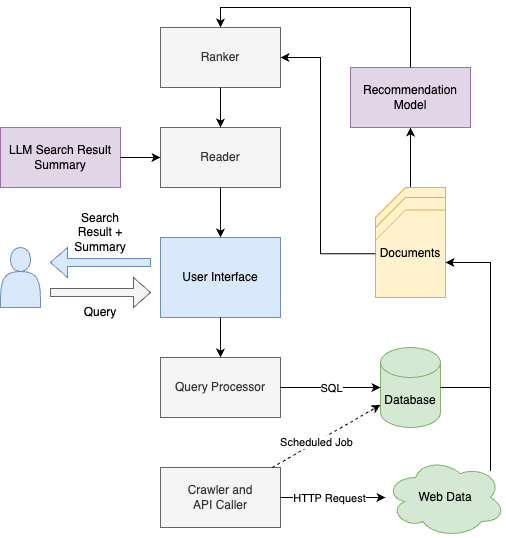
\includegraphics[width=1\linewidth]{doc//proposal//assets/sysarch.drawio_0319.png}
    \caption{System Architecture}
    \label{fig:sysarch}
\end{figure}

\begin{enumerate}
    \item  {User Interface}: The user interface consists of a search box for the user to type queries and an area to display search results (response). Most of the major front-end web development frameworks can provide the components we need. It is proposed that we use HTML + CSS + JavaScript as the project’s UI solution. Additional libraries and dependencies may be introduced in the engineering process.

    \item {Query Processor}: The query processor processes user input. There are three main tasks for the query processor. First, it uses LLM for keyword extraction if necessary. When the user puts their question in a sentence, we need the help of LLM to extract the keyword from the query. Spelling correction and query expansion will be taken into consideration. Then it constructs SQL queries to search for keywords in the database for local data retrieval.

    \item {Recommendation Model}: The input of the recommendation model is proposed to be a particular movie entry. It returns other similar movie entries based on the related algorithms that we proposed in the previous section. There are other potential methods to recommend movies, such as by returning movie guesses given a user profile or search history.

    \item {Ranker}: Ranker uses algorithms based on term frequency and weighting to sort the results. Users can also choose different ranking mechanisms such as relevance or date.

    \item {Reader}: Reader is a component where we gather all the relevant documents together and filter the repetitive documents. It constructs Movie entries from unstructured Documents and uses LLM to generate summary of the search result.

    \item {Crawler and API Integration}: The crawler and API caller will search for specific information for a movie entry, such as posters, and audience reviews. Wikipedia, for example, contains information about the plot and reception of the movie. Additionally, the crawler also runs regularly to update or insert entries to the database.

    \item {Large Language Model}: The model takes search result as input and generate a paragraph of summary of the result. We will experiment different tasks for the model to improve the performance. The problem defined in \textbf{Definition III.12} will also take advantage of the LLM.
\end{enumerate}


\section{Proposed Approaches}
\subsection{Data and Storage}
The following is the necessary aspects of our proposed system regarding data and storage as well as API integrating.

\subsubsection{Dataset}
The dataset used in the project is expected to include meta information about a movie, such as title, cast and genres. The metadata information will support the data retrieval function using query-document relevance algorithms. The dataset chosen for the project is \textbf{IMDb Non-Commercial Dataset}. The IMDb Non-Commercial Datasets offer subsets of IMDb's extensive data for personal and non-commercial use, with daily refreshes. This data is in tab-separated values (TSV) format with UTF-8 encoding. Each file begins with headers, using '\N' to indicate missing or null fields. Content include titles, their regional variations, basic metadata, crew details, episode information, principal cast and crew roles, and ratings, alongside basic information about individuals in the database. There are more than 1 million observations and 10 columns in the original dataset. Data prepossessing filtered out the non-English movies and movies that are too old. To insure scalability and usability of the system, we remained a majority of the observations and use popularity, the number of movie reviews, to control the corpus size. TSV files are processed by the means of Pandas and then inserted into relational database. The dataset was stripped of any missing values and irrelevant columns. 

\subsubsection{Backup Dataset}
Another approch is to use \textbf{MovieLens} dataset. For this project, the data sets must consist of metadata that can inform our system about each movie. This should consist of, title, actors, genre, year and reviews, etc. MovieLens is a widely recognized source with extensive metadata on movies. This dataset will provide a foundational source of data for the project, providing details basic details like overall user ratings on a scale of 0.5-5 stars. Additionally, MovieLens provides user profiles that are critical to our project's objectives. These profiles encompass user ratings, age, gender, geographical location, and occupation. Such information will be instrumental in clustering users with similar preferences to generate personalized movie recommendations.

\subsubsection{Database}
The entity relationship diagram in Figure 2, visualizes the database structure for the local data storage in our project. It details the "Movie" entity as the core, which includes attributes like movie ID, title, and release date. It is connected to "Actors" and "Directors" through associative entities "MovieActors" and "MovieDirectors," signifying many-to-many relationships, as a movie can have multiple actors and possibly multiple directors, and vice versa. There's also a "MovieGenres" associative entity that links movies to various "Genres," enabling films to be categorized into different genres, reflecting the possibility of a movie belonging to more than one genre. The data present in the database is from imdb’s open datasets\cite{IMDb}. 

\subsubsection{Updating Database}
The database is updated every 2 weeks after initial setup. The task of updating database is to download IMDb's new dataset and extract new entries. After filtering and API call, the database is considered synced with the new information.

\subsubsection{API Integrating}
The function of the API and Web Crawler is to provide our system with a substantial amount of data so our system can create and carry out recommendations and search queries. These search queries would be based on the user’s input and then the program will make the accurate call to the APIs used in this project. To enhance the text-based movie metadata, we made use of a third party service, TMDB API. Using the movie ID, which is the imDb id, we can send API calls to TMDB to retrieve the description of the movie. This is a piece of string typed information within 100 words for each movie. 

\subsection{Large Language Model}
The proposed Large language model for use in this project is going to be a local model. However, this is subject to change in the future depending on the capabilities of this LLM. As described in \textbf{Definition III.11}, LLM's main task is to summarize the search result of the system. The side task is to handle user's feedback.

\subsubsection{Model Properties}
The LLM used in our system “Vicuna-7b-v1.5”, which is an open-source chat assistant trained by fine-tuning Llama 2 on user-shared conversations collected from ShareGPT, this model contains approximately 7 billion parameters and outperformed the other LLMs, such as LLaMA and ALpaca, of the same scale\cite{zheng2023judging}. This model is available and can be downloaded at Hugging Face.  

\subsubsection{LLM Task Design}
In this checkpoint, our team tested the compatibility of this model in our system. Specifically, the task was to generate a description of a movie given an input of the title of the movie. In a proof-of-concept experiment, four movies were selected from the IMBD's Top 250 as the test case in this checkpoint\cite{IMDbhot250}. The titles of these movies are used as a vector of search results, which is a list of \(M\). The output of the model of each movie is shown in Fig~\ref{fig:llm}. 


\subsubsection{Model Performance Improvement}
Our team believes that the model is able to provide a decent description even with little prompting and it reaches our expectations. However, there are still two potential issues with the model: 1, we notice that the description of the movie “Saw” in the Fig. \ref{fig:llm} is much shorter than the other three movies. It is not clear why it happens, further tests and prompting may be needed to generate a longer and more detailed description. 2. Due to the nature of the model, it is not able to provide any information after its latest update. In this case, the model can not provide any description of a movie that is released later than the latest update of the LLM. 

\subsection{Recommendation System}
Due to the nature of the movie recommendation project,  our team plans to leverage both collaborative filtering and content-based filtering methods, which means we will recommend movies from two perspectives: the user's perspective, in which the recommendations are made based on the features of users (age, race, gender, etc). And the movie’s perspective, in which the recommendations are made based on the features of the movie (plot, cast, theme, etc). For the recommendation algorithms, our team proposes to use at least two machine learning-based methods: KNN and Principal Component Analysis (PCA). Other algorithms, such as neural networks or deep-learning algorithms, are also considered to be leveraged in this project.

\subsection{User Interface}
The user interface is an web application that allows the user to write queries based on their needs. The application will then implement the methods explained earlier, and provide users with exact results, and recommendations.

\begin{figure}
    \centering
    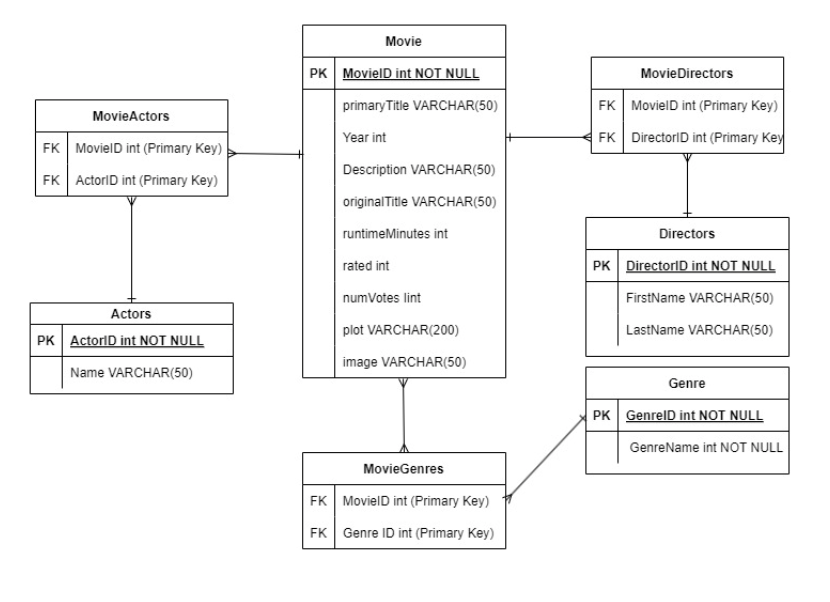
\includegraphics[width=1\linewidth]{doc//proposal//assets/erd.png}
    \caption{Entity Relationship Diagram}
    \label{fig:erd}
\end{figure}
\begin{figure}
    \centering
    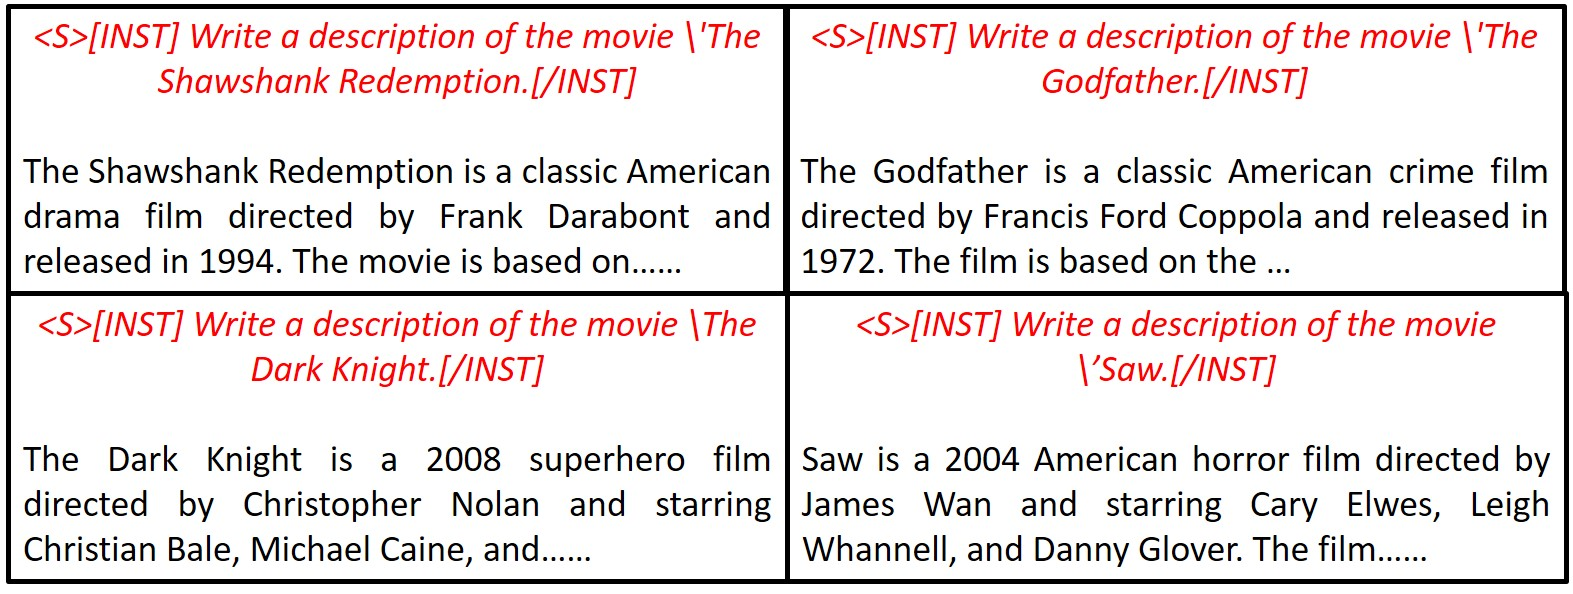
\includegraphics[width=1\linewidth]{doc//proposal//assets/llmresults.jpg}
    \caption{The input (the red and italics context at the top) and output (the black context) of the large language model. The full output of each movie test can be found in the appendix
}
    \label{fig:llm}
\end{figure}


% references section
\bibliographystyle{IEEEtran}
\bibliography{IEEEabrv, proposal-ref}

\section{Appendix}
\subsection{Timetable and Work Distribution for the Project}
This project is undertaken by a team comprising three members: Micah Harlan, Baiyi Zhang, and Jianger Yu. Each member is tasked with leveraging their specific expertise to contribute significantly to the project's completion. The project is organized into five distinct sections. As of March 19, 2024, the Data and Storage components, as well as the Application Programming Interface (API), have been successfully implemented. The forthcoming stages—namely the Large Language Model (LLM) and the Recommendation System—are scheduled for completion by April 9, 2024. The final phase, focusing on the User Interface (UI) development, is projected to be completed by May 7, 2024, thereby finalizing the application.

\subsection{Full Output of the LLM}
The complete output of the Large Language Model (LLM) is provided in the supplementary material section at the conclusion of this document.

\subsection{Screenshots of Database and Dataset}
The screenshot of the database as of the checkpoint 1 is provided in the supplementary material section at the end of this document.

\subsection{Progress Report}
In this progress report, we're detailing the contributions of each team member up to the current checkpoint.

Baiyi Zhang has completed the Design Overview and System Architecture, integrated the API into our project, and developed tasks for Large Language Models.

Micah Harlan has focused on the database aspect, designing the schema, creating the database itself, and handling dataset pre-processing.

Jianger Yu has been involved with the Large Language Models, setting them up, conducting tests on these models, and analyzing the results from these experiments.
\end{document}